\documentclass{beamer}

\mode<presentation>
{
  \usetheme{default}
  \usecolortheme{beaver}
  \setbeamercovered{transparent}
  \setbeamertemplate{caption}[numbered]
}

\usepackage{booktabs}
\usepackage{float}
\usepackage{siunitx}
\usepackage{subfloat}
\usepackage{subfig}
% \usepackage[labelsep=none,labelformat=empty]{caption}
\usepackage{caption}
% \usepackage{neuralnetwork}

\renewcommand{\tablename}{}
\newcommand{\ra}[1]{\renewcommand{\arraystretch}{#1}}

\title
{
    Gait Event Detection Using an LSTM Network
}

\subtitle
{
    10-701
    % Introduction to Machine Learning
    Project Presentation
}

\author
{
    Pablo Iturralde\\
    Yin Zhong\\
    Jakob Bauer
    % Pablo A. Iturralde,
    % Yin Zhong,
    % Jakob Bauer
}

\date
{
    April 22, 2015
}

% ==============================================================================

\begin{document}

\begin{frame}
  \titlepage
\end{frame}

\begin{frame}{Introduction}
    \begin{itemize}
        \item
            Goal: accurately detect gait events (heel strike, toe off) 
            in video-based motion capture data of human walking gait
        \item
            Necessary to analysis of changes in gait that arise from training,
            disease, aging, etc.
    \end{itemize}
    \begin{figure}
    \begin{center}
        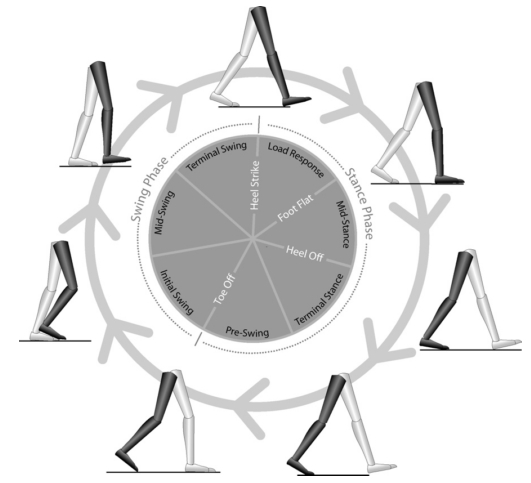
\includegraphics[width=0.5\textwidth]{figures/gait_events.jpg}
        \caption{Gait events [Rueterbories et al., 2010]}
        \label{fig:gait_events}
    \end{center}
    \end{figure}
\end{frame}

\begin{frame}{Data}
    \begin{itemize}
        \item All data are time series
        \item \textbf{Input:} 3D locus of 18 motion capture markers (54*N reals)
        \item \textbf{Output:}
        \begin{itemize}
            \item Raw: Event takes place $\Rightarrow$ 1; else $\Rightarrow$ 0 (4*N bools)
            \item Equivalent: Leg in stance phase $\Rightarrow$ 1; else $\Rightarrow$ 0 (2*N bools)
        \end{itemize}
        \item Training dataset:
        \begin{itemize}
            \item Sample rate: \SI{100}{\Hz}
            \item
                \num{240000} samples
                (8 subjects $\times$ 3 trials $\times$ \num{10000} samples)
            \item
                Ground truth from force plates on treadmills (very accurate)
        \end{itemize}
    \end{itemize}
\end{frame}

\begin{frame}{Baseline Methods}
    \begin{itemize}
        \item
            Signal processing approach [O'Connor et al., 2007]
            \begin{itemize}
                \item Heuristic based on position and speed of heel and toe markers
                \item \textbf{Pros:}
                \begin{itemize}
                    \item No training is needed
                    \item Good accuracy when input data is clean
                \end{itemize}
                \item \textbf{Cons:}
                \begin{itemize}
                    \item Sensitive to noise in input; resulting in gross mis-predictions
                    \item Need to manually specify sensitive thresholds
                    \item Heavy pre-filtering helps reduce noise but reduces accuracy
                \end{itemize}
            \end{itemize}
        \item
            Feed-forward Neural Network [Miller, 2009]
            \begin{itemize}
                \item
                    Sliding window centered around the desired marker
                \item \textbf{Pros:}
                \begin{itemize}
                    \item TODO %TODO
                \end{itemize}
                \item \textbf{Cons:}
                \begin{itemize}
                    \item Heavy preprocessing (dimensionality reduction, windowing, etc.); requires manual picking of parameters
                    \item TODO %TODO
                \end{itemize}
            \end{itemize}
    \end{itemize}
\end{frame}

\begin{frame}{Our Approach: LSTM}
    \begin{itemize}
        \item
            Motivation:
            \begin{itemize}
            \item
                Avoid manual picking of sensitive parameters (window size, threshold, filter cutoff, etc.)
            \item
                Human walking can be modeled as a dynamic system; RNN (Recurrent Neural Network) learns dynamic systems
            \item
                Any gait cycle may depend on ones preceding it
            \end{itemize}
        \item
            LSTM cell: RNN building block for variable time-dependence
        \item
            Network architecture:
            \begin{itemize}
                \item Inputs (54 reals)
                \item $n$ LSTM cells ($n$ reals in $[-1, +1]$)
                \item Output layer (softmax/sigmoid)
                \item Outputs ($2$ reals in $[0, 1]$)
            \end{itemize}
        \item
            Implementation:
            \begin{itemize}
                \item
                    Torch/Lua
                \item
                    LSTM cell by
                    de Freitas (Oxford University, Google Deepmind)
                \item
                    AWS EC2 GPU instance (g2.2xlarge)
            \end{itemize}
    \end{itemize}
\end{frame}

\begin{frame}{Results}
\end{frame}

\begin{frame}{Q\&A}
    \Large
    \centering
    Thank you for your attention!
\end{frame}

\begin{frame}{Network architecture}
    \begin{figure}[H]
        \begin{center}
        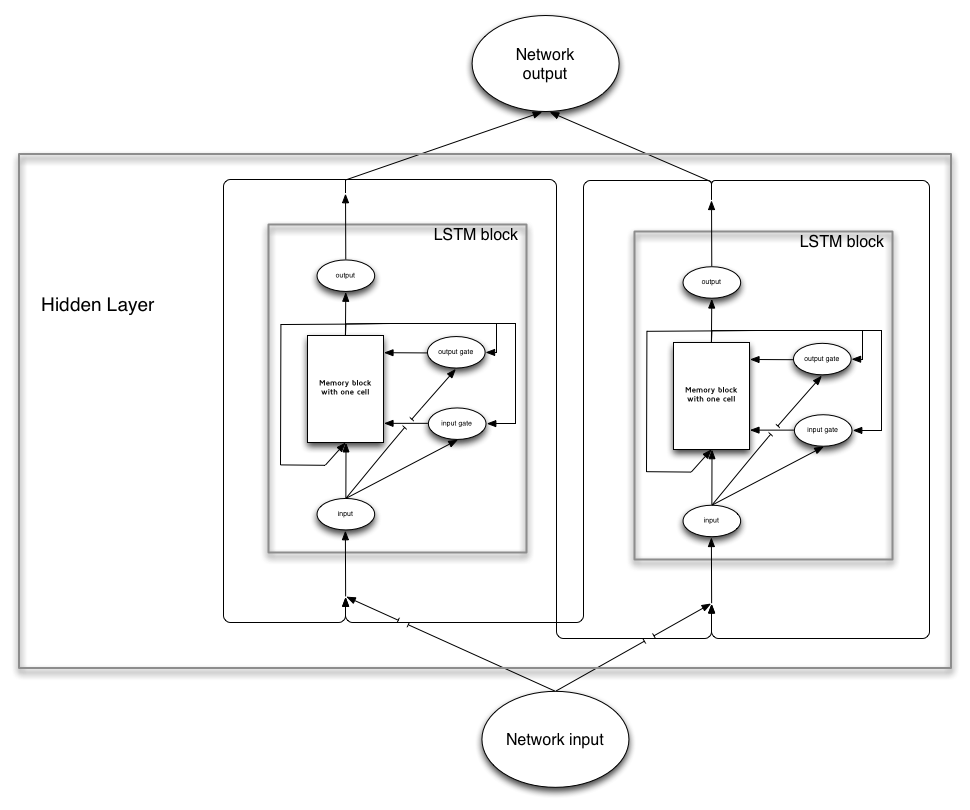
\includegraphics[height=.7\textheight]{figures/lstm2.png}
        \end{center}
    \end{figure}
\end{frame}
\begin{frame}{Lab setup (not our lab but similar)}
    \begin{figure}[H]
        \begin{center}
        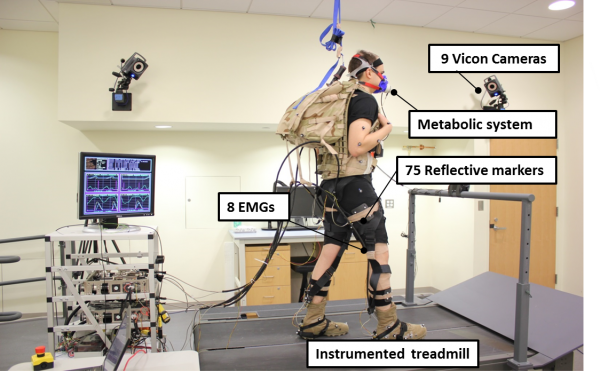
\includegraphics[height=.7\textheight]{figures/treadmill.png} \\
        \tiny from \url{http://biodesign.seas.harvard.edu/soft-exosuits}
        \end{center}
    \end{figure}
\end{frame}

\end{document}
